\documentclass{article}
\usepackage{tikz}
\usetikzlibrary{arrows.meta,positioning,calc,shapes.geometric}
\pagestyle{empty}
\begin{document}
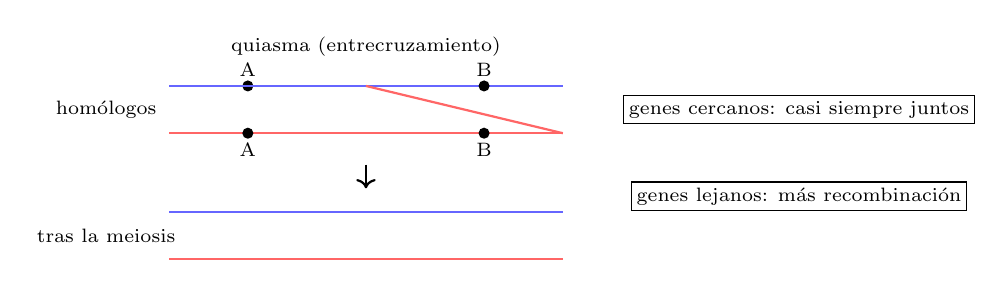
\begin{tikzpicture}

\draw[thick, blue!60] (0,2.2) -- (5,2.2); \draw[thick, red!60] (0,1.6) -- (5,1.6);
\draw[thick, blue!60] (0,0.6) -- (5,0.6); \draw[thick, red!60] (0,0) -- (5,0);
\node[font=\scriptsize] at (-0.8,1.9) {homólogos}; \node[font=\scriptsize] at (-0.8,0.3) {tras la meiosis};
\foreach \x/\l in {1.0/A, 4.0/B} {\fill (\x,2.2) circle (2pt) node[above, font=\scriptsize] {\l}; \fill (\x,1.6) circle (2pt) node[below, font=\scriptsize] {\l};}
\draw[thick, blue!60] (0,2.2) -- (2.5,2.2); \draw[thick, red!60] (2.5,2.2) -- (5,1.6);
\node[font=\scriptsize] at (2.5,2.7) {quiasma (entrecruzamiento)};
\draw[->, thick] (2.5,1.2) -- (2.5,0.9);
\node[draw, fill=white, font=\scriptsize, inner sep=2pt] at (8.0,1.9) {genes cercanos: casi siempre juntos};
\node[draw, fill=white, font=\scriptsize, inner sep=2pt] at (8.0,0.8) {genes lejanos: más recombinación};

\end{tikzpicture}
\end{document}
